\chapter{Configurations et transformations élémentaires du plan}
%\stepcounter{module}

{\AlegreyaSansLight \large
\begin{center}
\textbf{Crédit :} 46 heures\\
\textit{4 heures hebdomadaires}
\end{center}
}

\minitoc

\section{Introduction}

\subsection{Présentation du module}
Ce module comporte deux parties essentielles : les configurations planes, les symétries orthogonales et centrales dans le plan. Il développe deux compétences fondamentales que sont :
\begin{itemize}
\item déployer un raisonnement mathématique du type analogique, déductif et inductif ;
\item résoudre des problèmes par l'observation, l'identification et la caractérisation des formes planes ; par les transformations élémentaires que sont les symétries.
\end{itemize}
Il s'articule sur la famille de situations suivantes : représentations et transformations des configurations planes dans l'environnement. Les compétences mises en contexte s'appuient sur les trois catégories d'actions qui suivent :
\begin{itemize}
\item Reconnaissance des formes planes et des transformations dans l'environnement physique ;
\item Production des formes planes et transformations dans l'environnement physique ;
\item Détermination des mesures et des positions
\end{itemize}
Cette dernière catégorie d'actions est le champ privilégié de l'inter action entre les activités numériques et les activités géométriques de l'élève de 6ème.\\
Les différentes actions qui s'intègrent dans chacune des catégories suscitées sont en corrélation avec les savoirs essentiels que ce module développe, et qui s'appuient sur les habiletés cognitives suivantes : connaissance, compréhension et application.
\subsection{Contribution du module à la finalité et aux buts curriculaires}
A travers les différents raisonnements sus évoqués, l'apprenant développe les compétences transversales suivantes : le sens de l'ordre ; de la rigueur et de la concision ; le sens de l'initiative et de la créativité ; la pensée critique. Ils les développent en les intégrant, dans le cadre d'une démarche scientifique. Ces compétences contribuent à la formation d'un citoyen autonome et responsable dans l'exercice de ses rôles sociaux

\subsection{Contribution du module au programme d'études et aux domaines de vie}
La géométrie plane occupe une place privilégiée dans le programme de mathématiques de par les compétences qu'elle vise à développer. Sa contribution au développement de la technologie, de l'art, de la chimie, ne sont plus à démontrer. Enfin les innombrables symétries que la nature offre dans la biologie et la physiologie végétale ou animale font de ce module un des maillons essentiels dans plus d'un domaine d'apprentissage.\\
L'importance de ce module réside dans le fait que l'élève vit dans un espace géographique. L'utilisation et la rencontre des objets dans lesquels on peut extraire des formes géométriques planes font partie du quotidien : aménagement ou réalisation de son habitat, manipulation ou réalisation de certains objets usuels , appréciation ou production des œuvres d'art, choix du chemin adéquat pour se rendre à un lieu pour ne citer que celles-ci ; toutes choses pouvant l'aider à s'affirmer comme membre responsable d'une famille, à opérer des choix judicieux dans la consommation des biens , des services et de l'information. La contribution de ce module à tous les domaines de vie est donc d'une évidence incontestable.

\section{Matrice}

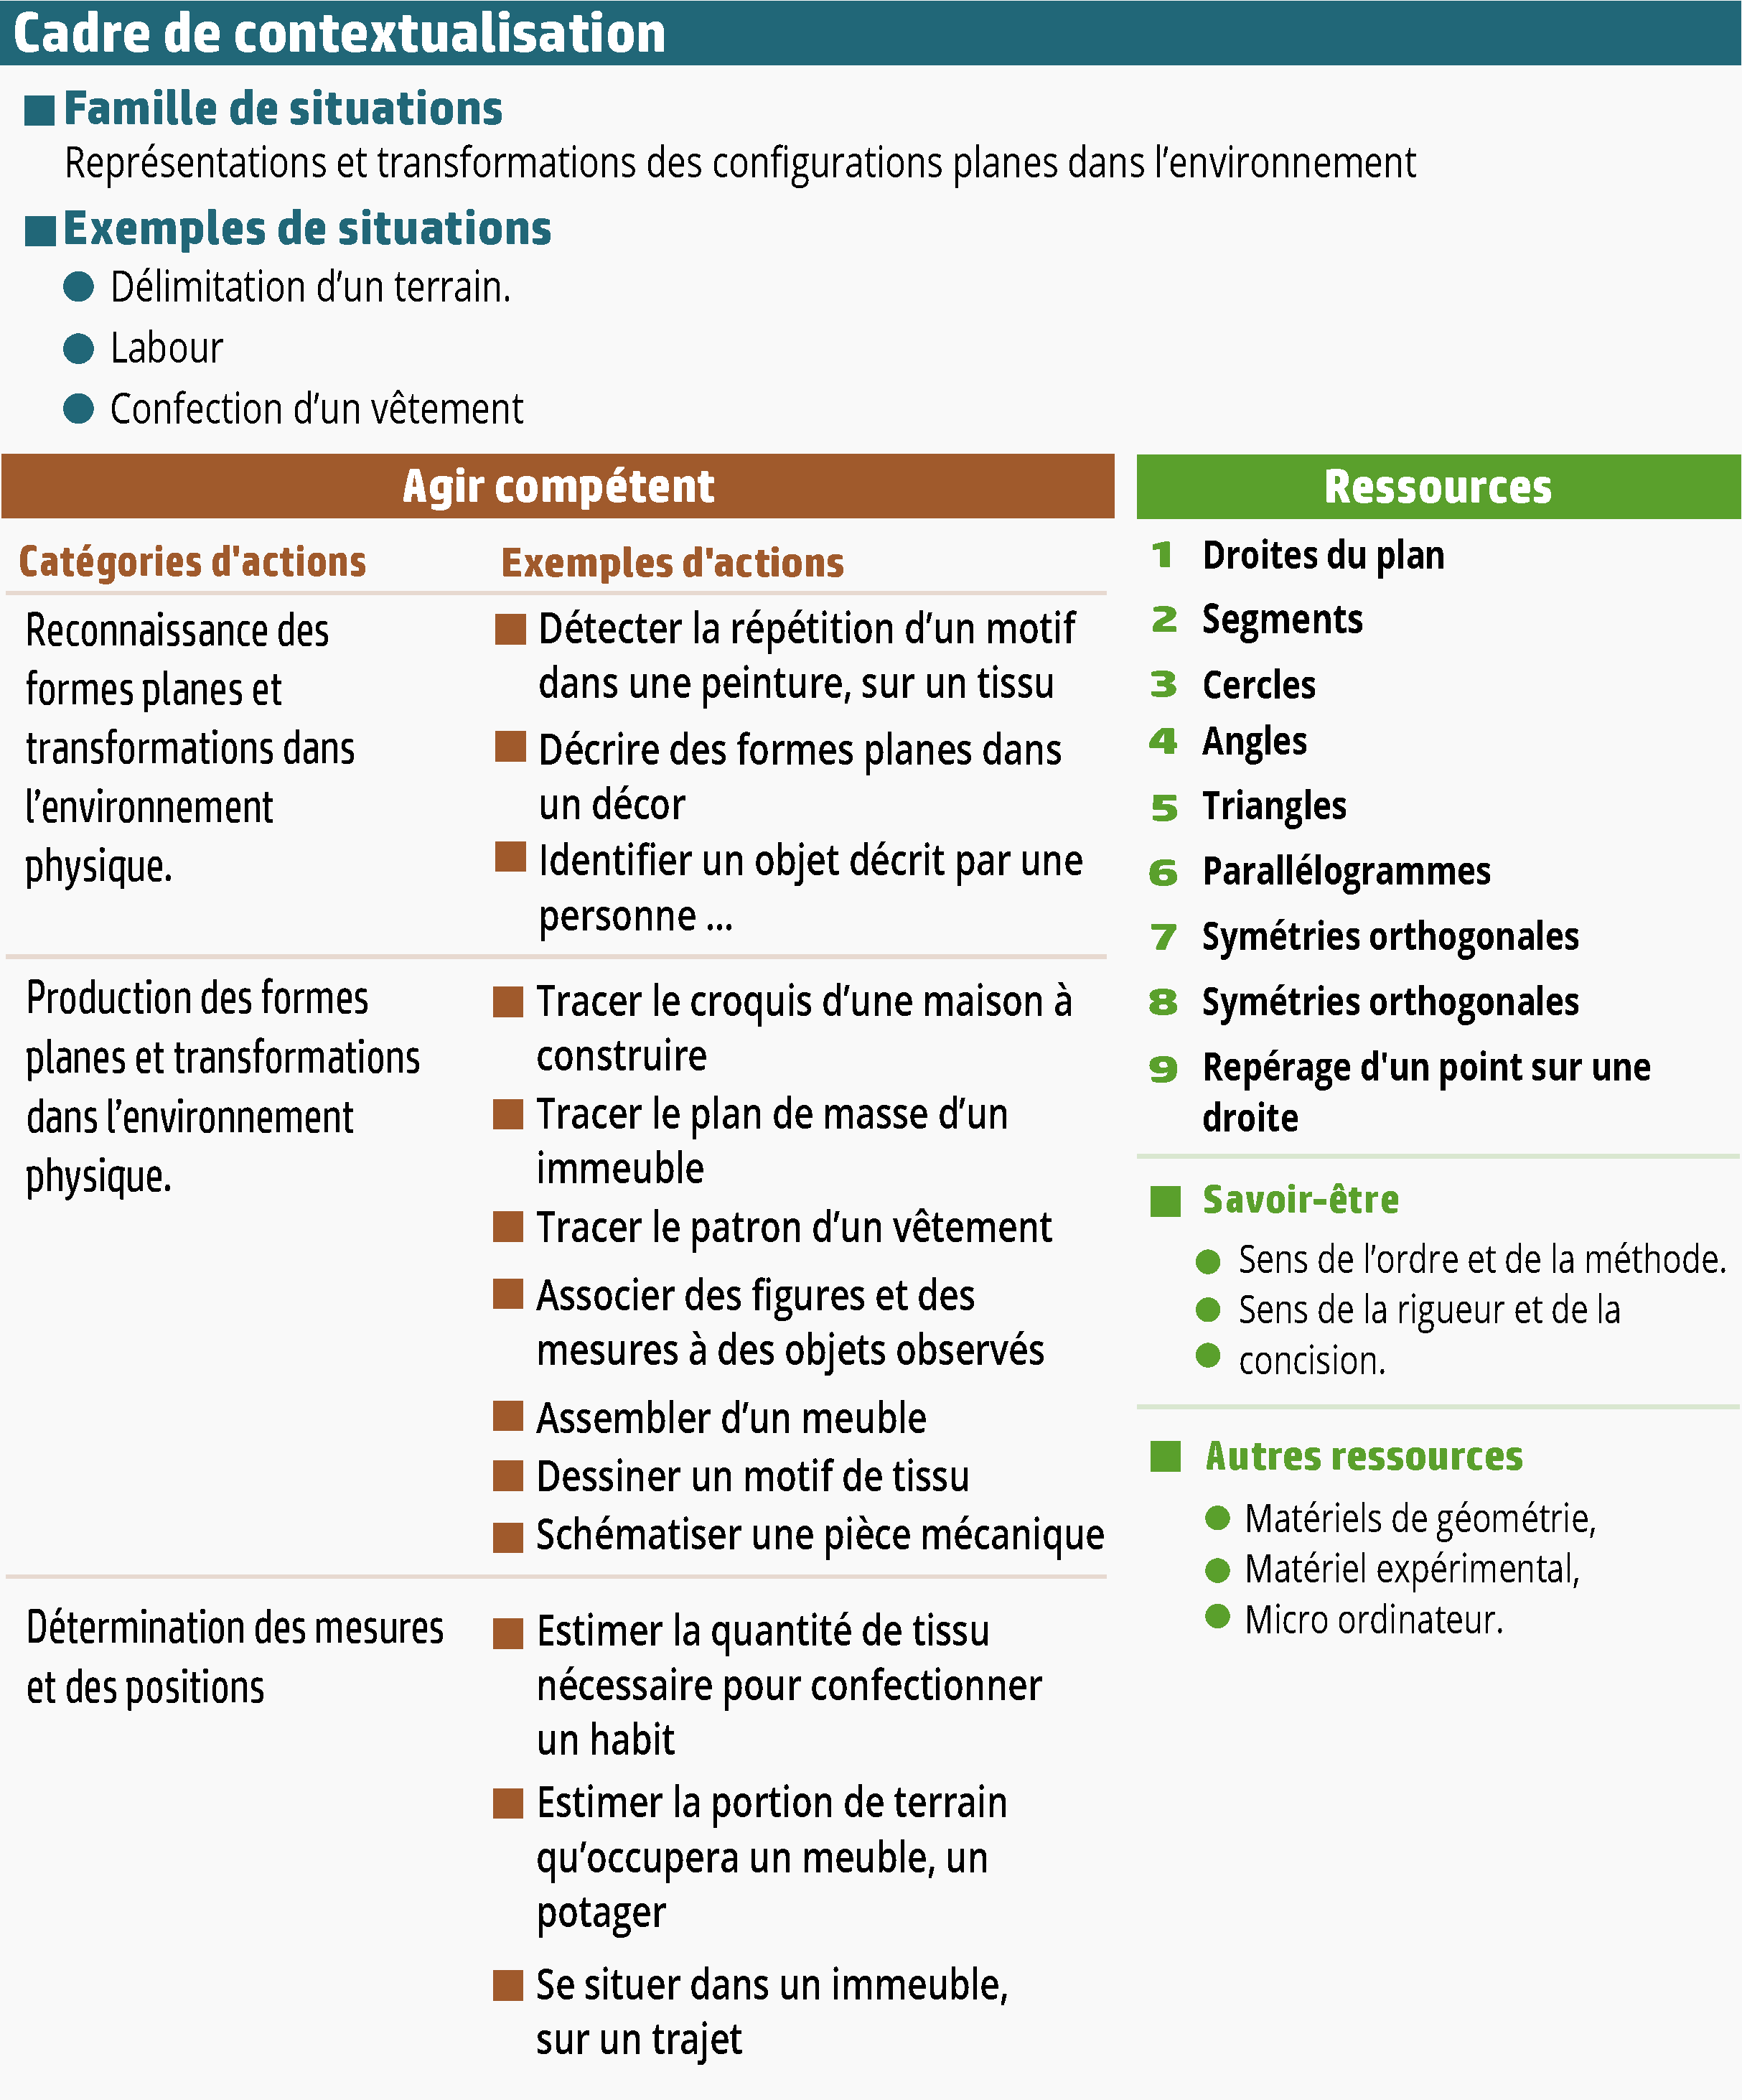
\includegraphics[scale=.36]{Module3.pdf} 

\subsection*{}
\addcontentsline{toc}{subsection}{\textbf{Ressource 1}: droites du plan}
\ressource{DP.pdf}

\savoir
\begin{itemize}
\item Droites : appartenance de points, notation, points alignés ;
\item Droites passant par :
\begin{itemize}
\item un point,
\item deux points distincts.
\end{itemize}
\item Régionnement du plan par une droite ;
\item Quatrième proportionnelle ;
\item Demi-droites ;
\item Droites sécantes;
\item Droites perpendiculaires :
\begin{itemize}
\item Symbolisme ;
\item \textit{Par un point donné, il passe une et une seule perpendiculaire à une droite donnée.}
\end{itemize}
\item Droites parallèles :
\begin{itemize}
\item Symbolisme ;
\item\textit{ Par un point donné, il passe une et une seule parallèle à une droite donnée ;}
\item \textit{Lorsque deux droites sont parallèles, toute parallèle (sécante, perpendiculaire)
à l'une est parallèle (sécante, perpendiculaire) à l'autre ;}
\item \textit{Deux droites perpendiculaires à une même droite sont parallèles.}
\end{itemize}
\end{itemize}
\savoirfaire
\begin{itemize}
\item Construction à l'aide des instruments (règle et équerre) :
Droite passant par 2 points, droite passant par un point et parallèle à une autre, droite passant un point et perpendiculaire à une autre.
\end{itemize}

\subsection*{}
\addcontentsline{toc}{subsection}{\textbf{Ressource 2}: segments}
\ressource{Seg.pdf}

\savoir
\begin{itemize}
\item Segments, support d'un segment ;
\item Longueur d'un segment ;\\
\textit{Propriété} : Si  $M\in\ife{AB}$ alors $MA+MB=AB$.
\item Milieu d'un segment ;\\
\textit{Propriété} : Si M est milieu du segment $\ife{AB}$ alors $MA=\dfrac{AB}{2}=MB$
\item Médiatrice d'un segment: définition.
\end{itemize}
\savoirfaire
\begin{itemize}
\item Construction de la médiatrice d'un segment à l'aide de la règle et de l'équerre ;
\item Construction d'un segment donné ;
\item Construction du milieu d'un segment donné à l'aide de la règle graduée;
\item Conversion des unités de longueur.
\end{itemize}

\newpage

\subsection*{}
\addcontentsline{toc}{subsection}{\textbf{Ressource 3}: cercle}
\ressource{Cer.pdf}

\savoir
\begin{itemize}
\item Rayon, diamètre, corde, arc, périmètre ou circonférence du cercle, disque, aire du disque ;
\item Positions relatives de deux cercles.
\end{itemize}
\savoirfaire
\begin{itemize}
\item Tracer un cercle de centre donné et de rayon donné ; 
\item Tracer un cercle de diamètre donné;
\item Calculer des éléments métriques (périmètre, aire, rayon, diamètre).
\end{itemize}

\subsection*{}
\addcontentsline{toc}{subsection}{\textbf{Ressource 4}: angles}
\ressource{Ang.pdf}

\savoir
\begin{itemize}
\item Notions d'angle et / ou de
secteur angulaire ;
\item \textit{Vocabulaire et notation}: sommet, côtés, angle saillant, nul, aigu, droit, obtus, plat, rentrant, plein ;
\item Mesures (en degrés) ;
\item Bissectrice.
\end{itemize}
\savoirfaire
\begin{itemize}
\item Construction d'un angle de mesure donnée ( à l'aide du rapporteur et de la règle) ;
\item Détermination de la mesure d'un angle donné ;
\item Construction de la bissectrice d'un angle donné à l'aide du rapporteur et de la règle. diamètre).
\end{itemize}

\subsection*{}
\addcontentsline{toc}{subsection}{\textbf{Ressource 5}: triangles}
\ressource{Tri.pdf}

\savoir
\begin{itemize}
\item Vocabulaire ;
\item Triangles particuliers ;
\item \textit{Droites particulières d'un triangle} : hauteur, médiane, bissectrice, médiatrice d'un côté ;
\item Périmètre et aire.
\end{itemize}
\savoirfaire
\begin{itemize}
\item Construction d'un triangle connaissant : les longueurs des côtés, la longueur de deux côtés et la mesure de l'angle qu'ils forment, la
longueur d'un côté et les mesures des angles à ses extrémités ;
\item Construction des triangles particuliers ;
\item Construction d'une hauteur, d'une médiane, d'une médiatrice, d'une bissectrice dans un triangle.
\item  Calcul du périmètre et de l'aire.
\end{itemize}

\subsection*{}
\addcontentsline{toc}{subsection}{\textbf{Ressource 6}: parallélogrammes}
\ressource{Par.pdf}

\savoir
\begin{itemize}
\item Parallélogramme, losange, rectangle, carré, périmètre et aire ;
\item \textit{Propriétés}: longueur des côtés opposés, diagonales, angles aux sommets opposés.
\end{itemize}
\savoirfaire
\begin{itemize}
\item Construction à l'aide du compas, de la règle et de l'équerre : du 4ème sommet d'un parallélogramme, d'un losange, d'un rectangle, d'un carré ;
\item Calcul de l'aire d'un parallélogramme, d'un losange, d'un rectangle, d'un carré;
\item Utilisation des propriétés pour justifier/déterminer une égalité de longueur, de mesure d'angle ;
\item  Techniques de conversion des unités d'aires.
\end{itemize}

\subsection*{}
\addcontentsline{toc}{subsection}{\textbf{Ressource 7}: symétries orthogonales}
\ressource{Syo.pdf}

\savoir
\begin{itemize}
\item Points symétriques par rapport à une droite.
\item \textit{Propriétés}: conservation de l'alignement, des longueurs, des angles, des formes.
\end{itemize}
\savoirfaire
\begin{itemize}
\item Construction du symétrique d'un point, d'une figure usuelle (segment, triangle, cercle, quadrilatères) par rapport à une droite. ;
\item  Utilisation des propriétés pour :
\begin{itemize}
\item justifier une égalité de longueur, de mesure d'angle ; 
\item déterminer une longueur, une mesure d'angle.
\end{itemize}  
\end{itemize}

\subsection*{}
\addcontentsline{toc}{subsection}{\textbf{Ressource 8}: symétries centrales}
\ressource{Syc.pdf}

\savoir
\begin{itemize}
\item Points symétriques par rapport à un point.
\item Propriétés: conservation de l'alignement, des longueurs, des angles, des formes.
\end{itemize}
\savoirfaire
\begin{itemize}
\item Construction du symétrique d'un point, d'une figure usuelle (segment, triangle, cercle, quadrilatères) par rapport à un point. ;
\item  Utilisation des propriétés pour:
\begin{itemize}
\item justifier une égalité de longueur, de mesure d'angle ; 
\item déterminer une longueur, une mesure d'angle.
\end{itemize}  
\end{itemize}

\subsection*{}
\addcontentsline{toc}{subsection}{\textbf{Ressource 9}: repérage d'un point sur une droite}
\ressource{Rep.pdf}

\savoir
\begin{itemize}
\item Demi-droite graduée, droite graduée ;
\item Origine, unité, abscisse d'un point, abscisse du milieu d'un segment.
\end{itemize}
\savoirfaire
\begin{itemize}
\item Placement d'un point d'abscisse donnée.  
\end{itemize}